\documentclass[a4paper,14pt]{extarticle}

\usepackage[utf8x]{inputenc}
\usepackage[T1,T2A]{fontenc}
\usepackage[russian]{babel}
\usepackage{hyperref}
\usepackage{indentfirst}
\usepackage{here}
\usepackage{array}
\usepackage{graphicx}
\usepackage{caption}
\usepackage{subcaption}
\usepackage{chngcntr}
\usepackage{amsmath}
\usepackage{amssymb}
\usepackage{pgfplots}
\usepackage{pgfplotstable}
\usepackage[left=2cm,right=2cm,top=2cm,bottom=2cm,bindingoffset=0cm]{geometry}
\usepackage{multicol}

\renewcommand{\le}{\ensuremath{\leqslant}}
\renewcommand{\leq}{\ensuremath{\leqslant}}
\renewcommand{\ge}{\ensuremath{\geqslant}}
\renewcommand{\geq}{\ensuremath{\geqslant}}
\renewcommand{\epsilon}{\ensuremath{\varepsilon}}
\renewcommand{\phi}{\ensuremath{\varphi}}

\counterwithin{figure}{section}
\counterwithin{equation}{section}
\counterwithin{table}{section}
\newcommand{\sign}[1][5cm]{\makebox[#1]{\hrulefill}} % Поля подписи и даты
\graphicspath{{pics/}} % Путь до папки с картинками
\captionsetup{justification=centering,margin=1cm}
\def\arraystretch{1.3}

\begin{document}

\begin{titlepage}
\begin{center}
	\textbf{Санкт-Петербургский Политехнический Университет \\Петра Великого}\\[0.3cm]
	\small Институт компьютерных наук и технологий \\[0.3cm]
	\small Кафедра компьютерных систем и программных технологий\\[4cm]
	
	\textbf{ОТЧЕТ}\\ \textbf{о лабораторной работе}\\[0.5cm]
	\textbf{<<Исследование частотных характеристик пассивных RC-цепей>>}\\[0.1cm]
	\textbf{Электротехника и Электроника}\\[10.5cm]
\end{center}

\begin{flushright}
	\begin{minipage}{0.60\textwidth}
		\begin{flushleft}
			\small \textbf{Работу выполнили студенты}\\[3mm]
			\small группа 23501/4 \hspace*{17mm} Дьячков В.В.\\[3mm]
			\small группа 23501/4 \hspace*{17mm} Ламтев А.Ю.\\[5mm]
			
			\small \textbf{Преподаватель}\\[5mm]
		 	\small \sign[3.5cm] \hspace*{8mm} к.т.н., доц. Кочетков Ю.Д.\\[0.5cm]
		\end{flushleft}
	\end{minipage}
\end{flushright}

\vfill

\begin{center}
	\small Санкт-Петербург\\
	\small \the\year
\end{center}
\end{titlepage}

\section{Цель работы}

Cравнение теоретических и экспериментальных характеристик фильтров,
проектирование и настройка фильтров высокого порядка, построенных на
операционных усилителях. 

\section{Чертеж схемы исследуемого устройства}

\begin{figure}[H]
\begin{center}
	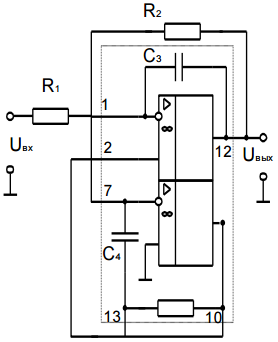
\includegraphics[width=0.4\textwidth]{scheme}
	\caption{Схема активного RC-фильтра 2 порядка}
\end{center}
\end{figure}

\section{Исходные данные}

\begin{table}[H]
\begin{center}
	\caption{Исходные данные}
	\def\tabcolsep{20pt}
	\begin{tabular}{|c|c|c|c|c|c|c|c|}
		\hline
		$f_{\text{м1}}$, Гц &
		$Q$ &
		$f_{\text{м2}}$, Гц &
		$Q$ &
		$\Delta L$, дБ \\
		\hline
		500 &
		5 &
		1000 &
		5 &
		6 \\
	    \hline	
	\end{tabular}
\end{center}
\end{table}

\section{Теоретические расчёты}

\subsection{First}

\begin{table}[H]
\begin{center}
	\caption{ЛАЧХ активного RC-фильтра 2 порядка}
	\label{tab:diff-int}
	\def\tabcolsep{20pt}
	\pgfplotstabletypeset[col sep=comma,
	    columns={f,u_in,u_out,k,lg_k},
	    column type/.add={|c|}{},
	    columns/f/.style={fixed, column name={$f$, Гц}},
	    columns/u_in/.style={fixed, precision=3	, zerofill, column name={$U_\text{вх}$, В}},
	    columns/u_out/.style={fixed, precision=3, zerofill, column name={$U_\text{вых}$, В}},
	    columns/k/.style={fixed, precision=3, zerofill, column name={$K$, В}},
	    columns/lg_k/.style={fixed, precision=3, zerofill, column name={$20 \cdot \lg K$, дБ}},
	    every nth row={1}{before row=\hline},
	    every head row/.style={before row=\hline, after row=\hline},
	    every last row/.style={after row=\hline}
	   ]{data/first.csv}
\end{center}
\end{table}

\begin{figure}[H]
\begin{center}
	\begin{tikzpicture} [every plot/.append style={thick}]
		\begin{axis}[
			height=0.45\textheight,
			width=0.95\textwidth,
			legend pos = north east,
			xlabel={$f$, Гц},
			ylabel={$20 \cdot \lg K$, дБ},
			axis x line = middle,
			axis y line = left,
			xmode=log,
			log basis x=2,
			xmin = 2^4,
			xmax = 2^14,
			ymin = -15,
			ymax = 35,
			grid=major
		]
		\addplot [smooth, mark=square*, blue] table[x=f,y=lg_k,col sep=comma]{data/first.csv};
		\legend{Эксп., Теор.}
		\end{axis}
	\end{tikzpicture}
	\caption{ЛАЧХ активного RC-фильтра 2 порядка}
	\label{plot:rectifier}
\end{center}
\end{figure}

\subsection{Second}

\begin{table}[H]
\begin{center}
	\caption{ЛАЧХ активного RC-фильтра 2 порядка}
	\label{tab:diff-int}
	\def\tabcolsep{20pt}
	\pgfplotstabletypeset[col sep=comma,
	    columns={f,u_in,u_out,k,lg_k},
	    column type/.add={|c|}{},
	    columns/f/.style={fixed, column name={$f$, Гц}},
	    columns/u_in/.style={fixed, precision=3, zerofill, column name={$U_\text{вх}$, В}},
	    columns/u_out/.style={fixed, precision=3, zerofill, column name={$U_\text{вых}$, В}},
	    columns/k/.style={fixed, precision=3, zerofill, column name={$K$, В}},
	    columns/lg_k/.style={fixed, precision=3, zerofill, column name={$20 \cdot \lg K$, дБ}},
	    every nth row={1}{before row=\hline},
	    every head row/.style={before row=\hline, after row=\hline},
	    every last row/.style={after row=\hline}
	   ]{data/second.csv}
\end{center}
\end{table}

\begin{figure}[H]
\begin{center}
	\begin{tikzpicture} [every plot/.append style={thick}]
		\begin{axis}[
			height=0.45\textheight,
			width=0.95\textwidth,
			legend pos = north east,
			xlabel={$f$, Гц},
			ylabel={$20 \cdot \lg K$, дБ},
			axis x line = middle,
			axis y line = left,
			xmode=log,
			log basis x=2,
			xmin = 2^5,
			xmax = 2^15,
			ymin = -15,
			ymax = 35,
			grid=major
		]
		\addplot [smooth, mark=square*, blue] table[x=f,y=lg_k,col sep=comma]{data/second.csv};
		\legend{Эксп., Теор.}
		\end{axis}
	\end{tikzpicture}
	\caption{ЛАЧХ активного RC-фильтра 2 порядка}
	\label{plot:rectifier}
\end{center}
\end{figure}

\subsection{Both}

\begin{table}[H]
\begin{center}
	\caption{ЛАЧХ активного RC-фильтра 4 порядка}
	\label{tab:diff-int}
	\def\tabcolsep{20pt}
	\pgfplotstabletypeset[col sep=comma,
	    columns={f,u_in,u_out,k,lg_k},
	    column type/.add={|c|}{},
	    columns/f/.style={fixed, column name={$f$, Гц}},
	    columns/u_in/.style={fixed, precision=3, zerofill, column name={$U_\text{вх}$, В}},
	    columns/u_out/.style={fixed, precision=3, zerofill, column name={$U_\text{вых}$, В}},
	    columns/k/.style={fixed, precision=3, zerofill, column name={$K$, В}},
	    columns/lg_k/.style={fixed, precision=3, zerofill, column name={$20 \cdot \lg K$, дБ}},
	    every nth row={1}{before row=\hline},
	    every head row/.style={before row=\hline, after row=\hline},
	    every last row/.style={after row=\hline}
	   ]{data/both.csv}
\end{center}
\end{table}

\begin{figure}[H]
\begin{center}
	\begin{tikzpicture} [every plot/.append style={thick}]
		\begin{axis}[
			height=0.45\textheight,
			width=0.95\textwidth,
			legend pos = north east,
			xlabel={$f$, Гц},
			ylabel={$20 \cdot \lg K$, дБ},
			axis x line = middle,
			axis y line = left,
			xmode=log,
			log basis x=2,
			xmin = 2^5,
			xmax = 2^14,
			ymin = -10,
			ymax = 40,
			grid=major
		]
		\addplot [smooth, mark=square*, blue] table[x=f,y=lg_k,col sep=comma]{data/both.csv};
		\legend{Эксп., Теор.}
		\end{axis}
	\end{tikzpicture}
	\caption{ЛАЧХ активного RC-фильтра 4 порядка}
	\label{plot:rectifier}
\end{center}
\end{figure}

\section{Экспериментально снятые зависимости}

\section{Погрешности}

\section{Выводы}

Приведённые погрешности полученных в ходе эксперимента значений $XXX$ не превышают предельно допустимые погрешности.

Таким образом, формулы \ref{eq:4:1} -- \ref{eq:4:6} являются верными.

\end{document}